\section{Aufbau und Durchf"uhrung}
	\label{sec:durchfuehrung}

	Zun"achst soll die Zeitabh"angigkeit der Amplitude einer ged"ampften Schwingung bestimmt werden.
	Hierf"ur wird ein Oszilloskop am Kondensator angeschlossen und ein Rechteckpuls in den RLC-Kreis gespeist.
	Der zeitliche Abstand zwischen zwei Pulsen muss gro"s genug gew"ahlt werden, damit eine Abklingen der Amplitude erkennbar ist, bevor die Schwingung neu angeregt wird.

	Anschlie"send wird der Widerstand $R_\mathrm{ap}$, bei dem der aperiodische Grenzfall eintritt bestimmt.
	Dazu wird der ohmsche Widerstand des Schaltkreises so gro"s gew"ahlt, dass ein reiner Kriechfall vorherscht.
	Unter beobachtung der Kondensatorspannung am Oszilloskop $U_\mathrm{C}$ wird der Widerstand verkleinert, bis das Signal fast einen Nulldurchgang, bzw. ein "Uberschwingen anzeigt.
	Der Widerstand $R_\mathrm{ap}$ ist dann gefunden.

	Daraufhin speist man die Schaltung mit einer Sinusspannung und misst die Kondensatorspannung $U_\mathrm{C}$ f"ur verschiedene Frequenzen $\omega$.
	Es ist wichtig, dass der Innenwiderstand des Sinusgenerators zum Gesamtwiderstand gerechnet wird.

	Schlie"slich wird die Phase in Abh"angigkeit der Frequenz gemessen.
	Dazu wird auch der Sinusgenerator am Oszilloskop angeschlossen und die Nulldurchg"ange beider Signale wie in Abbildung \ref{fig:phase} bestimmt.
	Es gilt dann

	\begin{equation*}
		\varphi = \frac{a}{b} 2 \pi
	\end{equation*}

	\begin{figure}[h!]
		\centering
		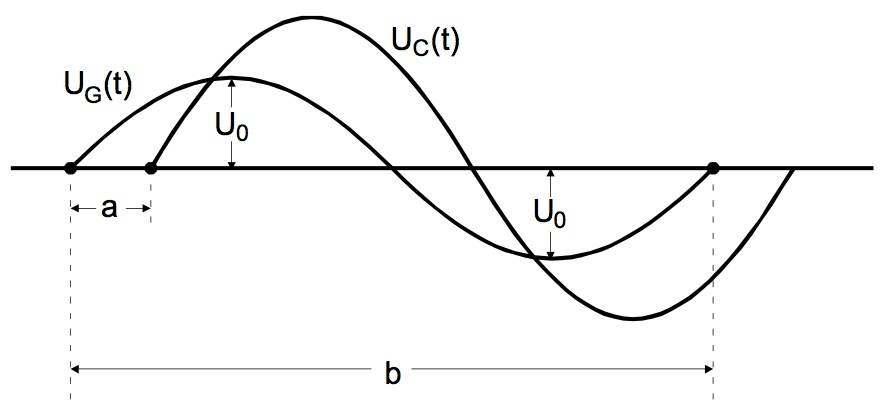
\includegraphics[width = 10cm]{img/phase.JPG}
		\caption{Bestimmung der Phase zweier Sinussignale. \cite{anleitung}}
		\label{fig:phase}
	\end{figure}